\documentclass[12pt]{article}

\usepackage{fullpage}
\usepackage{graphicx, rotating, booktabs} 
\usepackage{times} 
\usepackage{natbib} 
\usepackage{indentfirst} 
\usepackage{setspace}
\usepackage{grffile} 
\usepackage{hyperref}
\usepackage{adjustbox}
\setcitestyle{aysep{}}


\singlespace
\title{
\textbf{Reassessing the Public Goods Theory of Alliances}
	}
\author{Joshua Alley\footnote{Graduate Student,
Department of Political Science, Texas A\&M University.}}
\date{{\normalsize \today}}

\bibliographystyle{apsr}

\begin{document}

\maketitle 

\doublespace

\begin{abstract}
The public goods theory of alliances exerts substantial influence on scholarship and policy, but it has not received sufficient empirical scrutiny. 
The public goods model claims that smaller alliance participants can free-ride on larger partners because alliances face collective action problems. 
Prior statistical tests of free-riding suffer from identification and generalizability problems, so this study addresses those limitations. 
Using data on 285 alliances from 1816 to 2007, I examine whether economic weight in individual alliances is positively correlated with percentage changes in military spending. 
I find little evidence to support this alternative expression of the free-riding hypothesis. 
Therefore, the argument that alliances provide a public good and generate free-riding should be treated with more skepticism. 

\end{abstract} 

\newpage


%----------------------------------
\section{Introduction}



\citet{OlsonZeckhauser1966} argue that international alliances generate a collective action problem. 
According to their theory, security from an alliance is a public good, so smaller alliance participants ``free ride'' on the contributions of larger members. 
Free-riding is reflected by disproportionate allocations of resources to defense, where smaller alliance members spend a lower share of their national income on the military.
This view of alliances and defense effort is quite influential in scholarship \citep{Walt1990, Mearsheimer1994, Goldstein1995, SandlerHartley2001, Garfinkel2004, Walt2009, Norrlof2010, Barrett2010, PluemperNeumayer2015}. 


In addition, policy discussions of alliances employ collective action ideas.
Commentators and American policymakers often refer to allied ``free-riding.'' 
Thinking of alliance security as a public good and beset by collective action problems generates concern that the United States is ``being taken advantage of'' by junior partners. 
US policymakers often use free-riding and disproportionate contributions to the common good to criticize lackluster allied defense expenditures.  
For example, Barack Obama complained in 2016 that ``Free riders aggravate me'' and US allies ``have to pay your fair share.'' 
Donald Trump has implied the United States would not protect allies who spend too little on defense. 
Such complaints and exhortations go back as far as the Eisenhower administration \citep{Lanoszka2015}.


% this is the spot for Caverley's frame: debates about benefits and burdens of US Alliances 
Olson and Zeckhauser's argument has shaped a generation of policy and scholarly debate about alliances. 
Increasing great power competition makes assessing this theory even more important. 
Competing visions of US grand strategy hinge in part on the explanatory power of the public goods model. 
Advocates of retrenchment and ``restraint'' use the public goods logic to claim that US allies free-ride, so the United States should withdraw from many alliances \citep{Preble2009, Posen2014}. 
Others assert that alliances do not provide a public good and the benefits of alliance participation outweigh the costs \citep{Brooksetal2013, BrandsFeaver2017}. 


% So what am I doing here?: revisiting is necessary. 
The academic and policy salience of alliances and military spending means revisiting Olson and Zeckhauser's classic argument is worthwhile. 
In this paper, I reassess the public goods model by testing the extent of free-riding across 285 alliances. 
Revisiting the public goods model is necessary due to a major empirical shortcoming.
53 years after the publication of ``An Economic Theory of Alliances,'' there is little reliable and general evidence for or against Olson and Zeckhauser's prediction that small alliance members free-ride on larger partners. 


Existing tests of the public goods logic suffer from two key limitations.
First, many empirical estimates of free-riding within alliances are unidentified.
Olson and Zeckhauser measure defense burdens using military spending as a share of GDP and state size with GDP.
This approach is widely emulated, but it creates an identification problem because GDP is present on both sides of the equation.
There is a deterministic component in the relationship between GDP and defense burdens--- changes in GDP shift the defense burden.\footnote{
When GDP shifts, the defense burden remains constant only if military spending also changes in such a way that defense spending's share of GDP remains the same. Such changes are highly unlikely. Moreover, ratio dependent variables often generate spurious results \citep{Kronmal1993}.}  
 

One paper addresses the identification problem, but may not produce generalizable findings. 
\citet{PluemperNeumayer2015} examine how growth in military spending by North Atlantic Treaty Organization (NATO) members responds to changing US and Soviet spending.
They demonstrate that small NATO members are unresponsive to US and Soviet military spending, and present this as evidence of free riding.
\citet{PluemperNeumayer2015} find no correlation between NATO member size and the extent of free-riding, however, which they argue contradicts Olson and Zeckhauser.
The emphasis on NATO in this paper brings me to the second limitation: a lack of generalizability. 


% Huge (over)emphasis on NATO 
NATO is the epicenter of free-riding discussions. 
Following Olson and Zeckhauser's emphasis on military spending as a share of GDP, accusations of free-riding emphasize that NATO members have lower defense burdens than the United States. 
Scholars, pundits and policymakers have spent decades arguing over whether NATO members' defense burdens reflect free-riding \citep{SandlerForbes1980, Palmer1990, Boyer1993, GatesTerasawa1992, SandlerHartley2001, Lanoszka2015, PluemperNeumayer2015}.


% So what is the problem here?: it's mostly NATO
Most studies of the public goods model focus on NATO, but NATO is a difficult case from which to draw general conclusions because it is exceptional. 
NATO is exceptionally large, durable and capable. 
There are only seven tests of alliance free-riding outside of NATO, all of which examine a few alliances \citep{Russett1970, Starr1974, Reisinger1983, Thies1987, ConybeareSandler1990, OnealWhatley1996, Siroky2012}. 
Six of these studies include GDP in the independent and dependent variable, so they suffer from the aforementioned identification problem.
The seventh study uses case comparisons.
Thus, there is still need for a general examination of the public goods logic. 


Here, I address the identification and generalizability issues in a test of the public goods model.  
I use the public goods logic to predict a positive correlation between states' economic weight in their alliances and percentage changes in military spending. 
Then I employ a Bayesian model to estimate the association between economic weight and percentage changes in military spending across 285 alliances. 
I find no alliances with a clear positive correlation between economic weight and military spending. 


% I'm not the first one to address this theory: first comprehensive empirical evidence
My findings will not surprise skeptics of the public goods model of alliances. 
Many already question the public goods theory of alliances on theoretical grounds \citep{Palmer1990, GatesTerasawa1992, SandlerHartley2001, Norrlof2010, NiouZeigler2019}.
But absent a reliable and general test, theoretical revisions of a parsimonious public goods model may be inappropriate.
Accurate assessment should proceed dismissing or modifying the public goods model. 
Revisiting the pure public goods logic and clarifying its empirical value can then refine theories of alliances. 


% note that evidence against has same reliability problem
Skeptics may also argue that we already know there is little empirical support for the public goods model. 
The limits of existing tests also apply to this claim, however. 
The general findings in this paper provide new evidence about the explanatory power of the public goods model. 


The paper proceeds as follows.
First, I summarize the public goods theory of alliances and derive an observable implication of free-riding from it.
Then, I describe the model and results from testing the prediction. 
The final section assesses implications for scholarship and policy. 



\section{Free-Riding in Alliances}

% New para clarifying that I do not test their exact proposition 
To identify a testable implication of free-riding, I use the public goods argument, but make a slightly different prediction.
This theoretical exercise does not critique the public goods model.
Instead, I take the public goods logic as given and generate an alternative expression of the key claim that small states free-ride. 
Following \citet{PluemperNeumayer2015} I use percentage changes in military spending to conceptualize defense effort.
I then assess the role of relative state size using economic weight. 


% summarize argument
Why might alliances suffer from a collective action problem?
The aggregate military capability of an alliance provides security for members and states contribute by investing in their military.
Because an alliance cannot exclude members without undermining its purpose, alliance security is a public good. 
Alliance members receive security regardless of their individual contribution.\footnote{The marginal costs and benefits of participation depend in part on group size, but Olson and Zeckhauser's model shows free-riding even in a bilateral alliance.}
Thus, states have incentives to rely on their alliance partners to contribute military capability and reduce their own military expenditures.  

 
Olson and Zeckhauser expect that larger members of the alliance will bear a higher defense burden, because these states value security from the alliance more.
Small alliance members rely on the contributions of larger partners for security and bear a lower defense burden.
As a result, smaller states free-ride on larger alliance participants. 
Moreover, smaller states have greater bargaining leverage, because a large state cannot credibly threaten to reduce their contribution and has ``relatively less to gain than its small ally from driving a hard bargain'' \citep[pg. 274]{OlsonZeckhauser1966}. 


% Economic weight as another way to get at O+Z's key comparion
Olson and Zeckhauser compare alliance members using economic resources, specifically GDP.
Economic weight within an alliance, or each state's share of total allied GDP, is a related way to conceptualize differences in state size.\footnote{Different states may be large or small relative to their allies, depending on treaty membership.} 
Using economic weight facilitates comparisons of state size across diverse alliances. 
A greater share of total economic resources in an alliance gives a state more economic weight and increases their potential contribution of military spending. 


Because Olson and Zeckhauser expect that large states contribute disproportionately to an alliance, economic weight shapes defense expenditures. 
Inasmuch as larger states value security from an alliance more, alliance participation will increase their investment in military capability.
Smaller members can free-ride through lower military spending. 
Therefore, the share of total allied GDP and percentage changes in military spending will be positively correlated. 


\begin{quote}
\textsc{Hypothesis 1}: As a state's share of total GDP in an alliance increases, annual percentage changes in military spending will increase. 
\end{quote}


A positive correlation between economic weight and military spending suggests free-riding in an alliance. 
More alliances with this correlation imply more cases where the public goods argument has some explanatory power. 
A negative correlation between economic weight and military spending implies that larger members have lower spending. 
To look for general evidence of free-riding, I assess how many alliances have a positive correlation between shares of total allied GDP and military spending.  
 

% Clarify that both predictions approximate the O+Z logic
Hypothesis 1 approximates Olson and Zeckhauser's prediction that smaller alliance members will spend a smaller share of their economic resources on the military. 
Though my prediction is different, it facilitates a reliable and general empirical test.
I now test Hypotheses 1 in a sample of all non-microstates with at least one alliance from 1816 to 2007.
Analyzing states in alliances limits comparisons to alliance participants and places more weight on within-treaty differences. 
State-year observations are the unit of analysis.


\section{Testing Hypothesis 1}


Hypothesis 1 predicts the association between economic weight and military spending for individual alliances. 
For each of the 285 alliances that promise military support,\footnote{ATOP offensive and defensive treaties \citep{Leedsetal2002}.} I estimate a parameter measuring the correlation between economic weight and military expenditures. 
This model examines alliance free-riding using evidence from many treaties.\footnote{I also regress percentage changes in military spending on state's average weight in their alliances, and make similar inferences, which I report in the appendix.}
Bayesian estimation regularizes estimates with many parameters, so I fit the following model using STAN \citep{Carpenteretal2016}.


The model starts with state-year percentage changes in military spending $y_{it}$, transformed with an inverse hyperbolic sine.
I model this variable as a t-distribution with degrees of freedom $\nu$ to account for heavy tails.
The expected value of military spending $\mu_{it}$ depends on a constant $\alpha$, state and year varying intercepts, and control variables $\mathbf{X_{it}} \beta$.\footnote{See the appendix for a full description of all the variables in the model.} 
\begin{equation}
y_{it} \sim student_t(\nu, \mu_{it}, \sigma) 
\end{equation}

\begin{equation}
\mu_{it} = \alpha + \alpha^{st} + \alpha^{yr} + \mathbf{X_{it}} \beta + \mathbf{Z_{it}} \gamma
\end{equation}


The $\mathbf{Z_{it}} \gamma$ term captures the impact of economic weight in alliances.  
\textbf{Z} is a matrix of state participation in alliances--- columns are alliances, rows are state-year observations.  
If a state is part of an alliance, the associated matrix element is equal to a state's GDP as a share of total GDP in the alliance.\footnote{All GDP values are logged.} 
If a state is not part of an alliance, the corresponding matrix element is zero. 


\textbf{Z} is a quasi-spatial approach to capturing the impact of participation in multiple alliances.
Alliance participation affects military spending through economic weight in this model.  
The $\gamma$ parameters capture the correlation between economic weight in an alliance and military spending. 


$\gamma$ is a vector of 285 alliance-specific parameters.  
Because \textbf{Z} contains each state's share of allied GDP, these coefficients estimate the association between economic weight and military spending.\footnote{I multiply the vector $\gamma$ and the ragged matrix $Z$ by using alliance indexes to match elements of $\gamma$ with the corresponding columns of $Z$ for each observation.} 
When a state is not in an alliance, the corresponding $\gamma$ is multiplied by zero, and has no impact. 


Each alliance has a separate impact on military spending.
While these alliance parameters are distinct, they have a common prior distribution.
Partial pooling estimates the dispersion of the alliance parameters from the data, so the prior for $\gamma$ is normally distributed with mean $\theta$ and variance $\sigma_{all}$. 
$\theta$ is the mean hyperparameter of the alliance coefficients and each $\gamma$ deviates from $\theta$ based on the variance hyperparameter $\sigma_{all}$.
Every alliance estimate holds the impact of other treaties constant. 
A positive $\gamma$ implies that alliance members with more economic weight have higher percentage changes in military spending, as Hypothesis 1 predicts. 
    


\subsection{Results} 


Hypothesis 1 predicts many positive $\gamma$ parameters. 
Because I employed Bayesian modeling, each $\gamma$ has a posterior distribution.\footnote{See the appendix for a full summary of priors, convergence and model fit. I also show that the model can recover known parameters from simulated data.} 
I focus interpretation on the posterior mean and 90\% credible intervals.\footnote{I use 90\% credible intervals because inferences around 95\% intervals are less stable. The 90\% credible interval falls between the 5\% and 95\% quantiles of the posterior.}
The posterior mean is the expected value of $\gamma$, while the credible intervals capture uncertainty around that estimate.  


\autoref{fig:alliance-coefs-year} plots the $\gamma$ parameter for each alliance against the start year of the treaty.
Points mark the posterior mean. 
The error bars encapsulate the 90\% credible interval.


\begin{figure}[htbp]
	\centering
		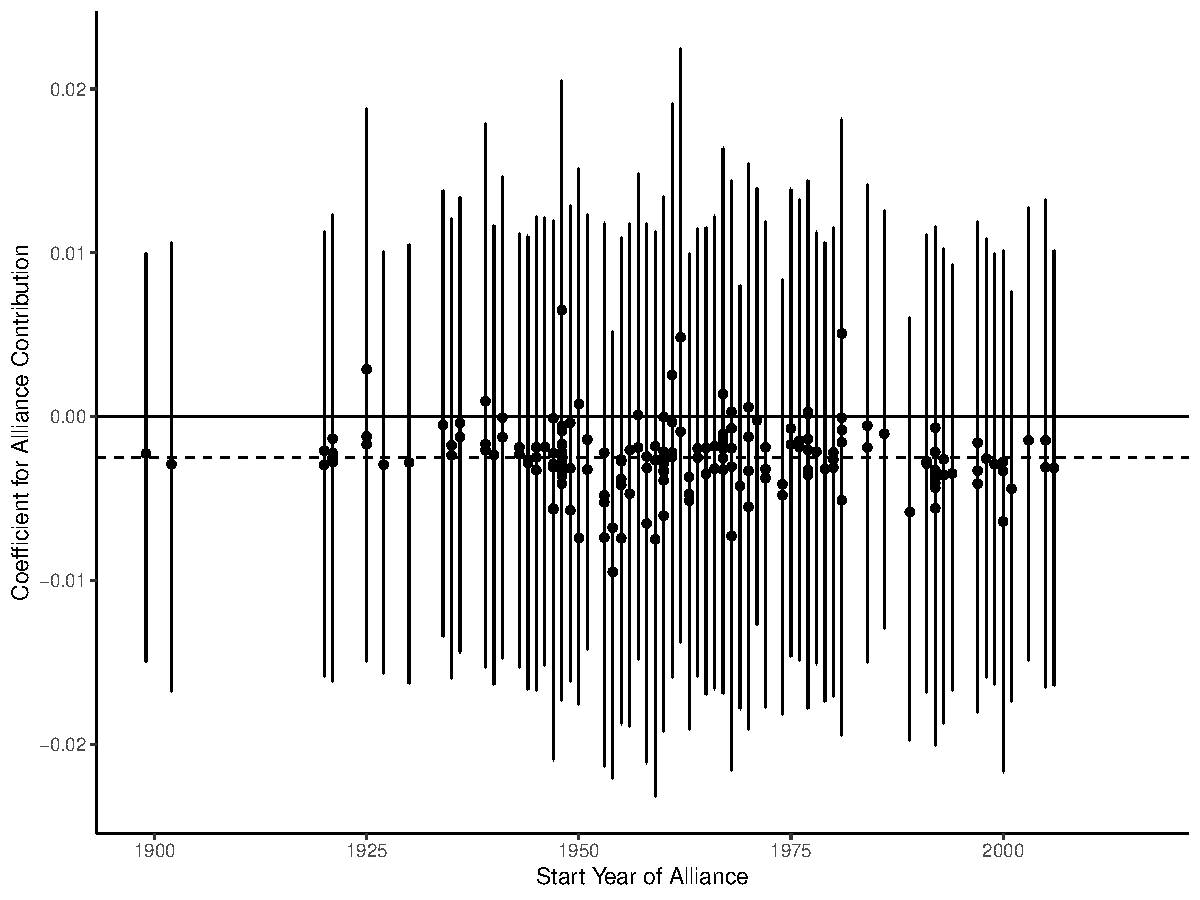
\includegraphics[width=0.95\textwidth]{alliance-coefs-year.pdf}
	\caption{Estimated association between share of total allied GDP and defense spending in 285 defensive and offensive alliances from 1816 to 2007. Points represent the posterior mean and the error bars cover the 90\% credible interval. The dashed line marks the posterior mean of the $\theta$ parameter, which represents the average association between economic weight and percentage changes in military spending.}
	\label{fig:alliance-coefs-year}
\end{figure}


All 285 alliances have a negative posterior mean and all the 90\% credible intervals overlap zero. 
Most credible intervals are consistent with effects ranging from -0.03 to 0.02. 
There is not a preponderance of positive coefficients. 


As \autoref{fig:alliance-coefs-year} shows, partial pooling of the $\gamma$ parameters strongly regularizes these estimates. 
$\theta$ has a posterior mean of -0.007, which is close to zero. 
The effects of increasing economic weight $\gamma$ are tightly clustered around the mean hyperparameter. 
Under these circumstances, it is difficult to distinguish any estimates from zero, even as partial pooling shares information across coefficients and reduces uncertainty. 


The small scale of the $\gamma$ parameters is reflected in predictions of how changing a state's share of allied GDP alters military spending. 
To assess whether increasing a state's share of allied GDP leads to higher defense spending, I simulated the effect of changing economic weight on percentage changes in military spending. 
In the simulated data, I used the full posteriors of the intercept $\alpha$, all the $\beta$ coefficients, and one $\gamma$ parameter. 
I selected the $\gamma$ parameter with the most positive posterior mass, so this simulation is the \emph{best case} for Hypothesis 1. 
I set the state-level regressors at their median value and varied economic weight between minimum (0.02), median (0.2) and near maximum (0.7) values. 


In \autoref{fig:pred-change-share}, I summarize predicted changes in military spending at different levels of economic weight. 
In this figure, the point marks the mean and the error bars summarize the 90\% credible interval. 
Though moving from the minimum share of allied GDP to the high value of .70 slightly decreases the median value, the three predictions are indistinguishable. 
There is no evidence that increasing economic weight leads to higher military spending. 

\begin{figure}[htbp]
	\centering
		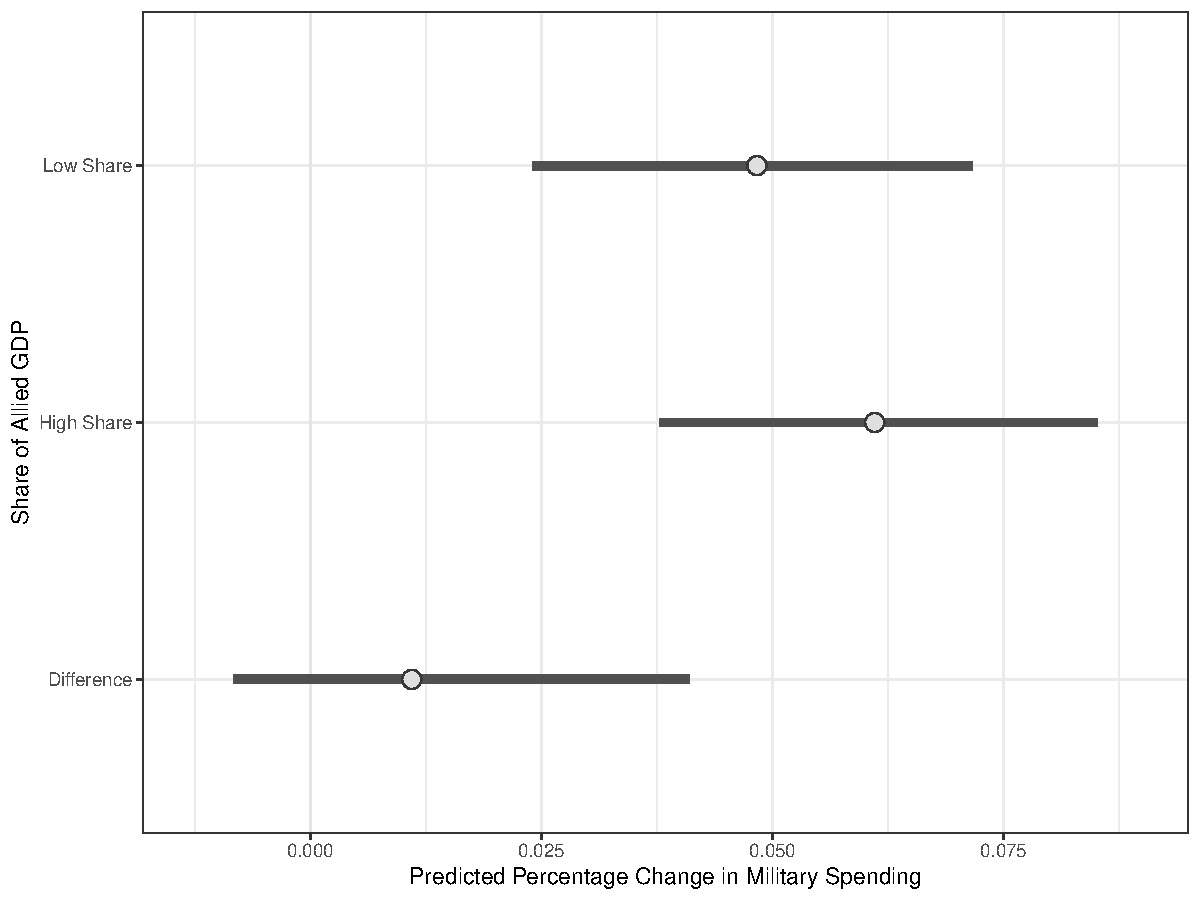
\includegraphics[width=0.95\textwidth]{pred-change-share.pdf}
	\caption{Predicted percentage changes in military spending for a simulated state with minimum, median and high shares of total allied GDP. Points mark the median value, and the error bars summarize the 90\% credible interval.}
	\label{fig:pred-change-share}
\end{figure}


The $\gamma$ estimates also produce inferences about individual alliances.
The estimated $\gamma$ for NATO offers no support for the public goods theory of alliances. 
The posterior mean of this parameter is $-0.007$, and the credible interval ranges from -.03 to .01.  
A greater share of NATO's total GDP has no clear association with percentage changes in military spending. 
This finding corroborates the size result of \citet{PluemperNeumayer2015}, but NATO members may still spend less on the military as allied capability changes \citep{GeorgeSandler2017}.


\section{Conclusion}

% Add paragraph summarizing results
There is little evidence that small alliance members free-ride on their partners. 
These findings should increase our skepticism about the public goods model of alliances. 
Although Olson and Zeckhauser's model is parsimonious, it lacks explanatory power. 
Estimates from multiple treaties produce little evidence to match predictions from the public goods logic. 


The best theoretical alternative to the public goods approach emphasizes exchange between alliance members and intra-alliance bargaining \citep{Norrlof2010, Brooksetal2013, Kim2016}. 
If large and small states use alliances for distinct purposes, alliance members can trade different foreign policy goods \citep{Morrow1991, Johnson2015}. 
Small states might use alliances for immediate territorial security. 
Large states could be more focused on using alliances to defend other states and expand their influence abroad. 


Scholars and policymakers should reassess the way they use ``free-riding'' to describe alliance politics. 
Free-riding is inextricable from a public goods understanding of alliances.
But if the public goods model has little empirical support, free-riding is an inaccurate description of reduced defense effort by alliance participants.  
Charges of free-riding may mask exchange between alliance members \citep{Lanoszka2015}. 


Scholars should not abandon the public goods model in international politics, however.   
Using alliances as exemplars of collective action problems in other international organizations is inappropriate, but collective action can apply to other international organizations. 
Thinking about alliances using exchange may be more fruitful than the collective action problem envisaged by Olson and Zeckhauser, so policymakers and scholars should exercise caution in using to the public goods model to understand alliance politics.  



\singlespace


\bibliography{../../../MasterBibliography} 





\end{document}

